% Benchmark
% task formulation 
% data curation
% metrics
% Perception – [which is better] ✅
% Similarity – [video, slides+subtitle, speech] ✅
% Performance - [video QA] ✅
% Ablation experiments
% talking-head&personalized speech – [needle in a haystack] ✅
% 4 video clips + 4 qa & querry image or audio
% cursor (?)
% user study on w/o cursor, w/o talking-head, w/o personalized speech
% 导言区:
% \usepackage{graphicx}
% \usepackage{subcaption}

% 导言区:\usepackage{graphicx}\usepackage{subcaption}



% \section{\our~Benchmark}
% \begin{figure}[t]
%     \centering
%     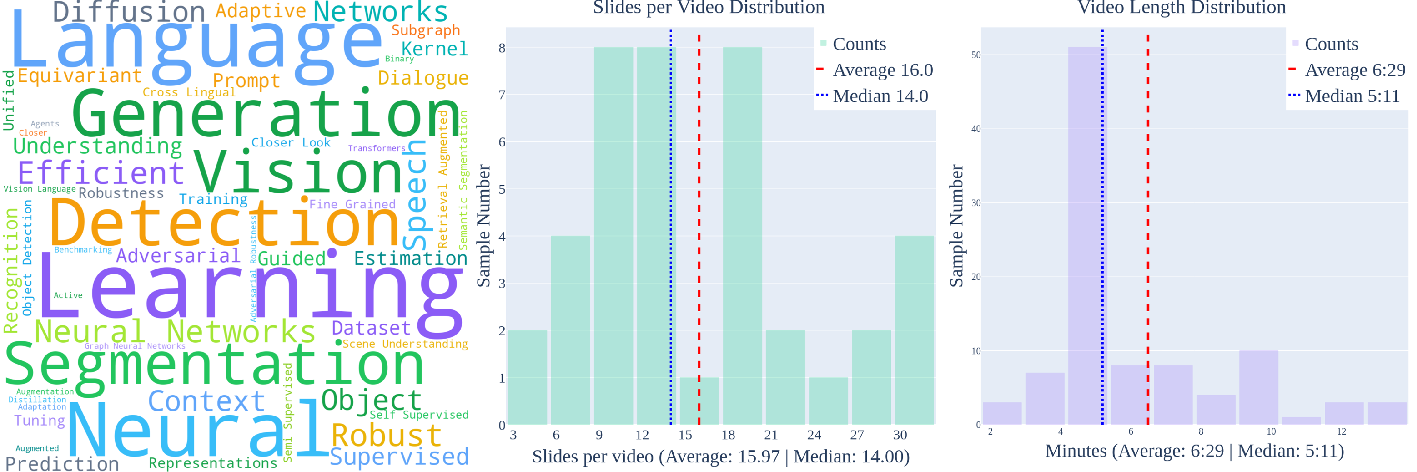
\includegraphics[width=\linewidth]{figure/data_stat.pdf}
%     \caption{Overview of Paer2Video benchmark.\kevin{all pdf; by three separate fig;}}
%     \label{fig:data_stat}
% \end{figure}
\vspace{-0.2\baselineskip} 
\section{\bench~Benchmark}
\vspace{-0.4\baselineskip} 
\subsection{Task Definition}
\vspace{-0.4\baselineskip} 
% \kevin{slightly longer}
Given a research paper and the author’s identity information, our goal is to automatically synthesize an academic presentation video that faithfully conveys the paper’s core contributions in an audience-friendly manner. 
We identify that a perfect presentation video is usually required to integrate four coordinated components: 
\textbf{(\textit{i}) slides} contain well-organized, visually oriented, expressive figures and tables with concise text description;
%\kevin{well-organized content, visually rather than dense text}
\textbf{(\textit{ii}) synchronized subtitles and speech} are semantically aligned with the slides, including supplementary details;
% \kevin{is usually not exactly the same as slide}
\textbf{(\textit{iii}) presenter} should exhibit natural yet professional facial expressions, ideally accompanied by appropriate gestures;
% \kevin{encourage to show face, sometimes gesture}
and \textbf{(\textit{iv}) a cursor indicator} serves as an attentional anchor, helping the audience focus and follow the narration.
%kevin{that anchors visual attention, helps the audience to focus}. 

\vspace{-0.2\baselineskip}
This task poses several distinctive challenges: 
\textbf{\textit{a}. Multi-modal Long-Context Understanding.} Research papers span many pages with dense text, equations, figures, and tables.
% Generating formal, well-structured slides with fine-grained layout requires content selection, cross-modal grounding, and fine-grained layout design. 
\textbf{\textit{b}. Multi-turn Agent Tasks.} It is challenging to solve this task with a single end-to-end model, as it requires multi-channel generation and alignment (\textit{e.g.}, slides, cursors, and presenter). 
%An efficient, well-designed agent system is therefore needed to address this task.
\textbf{\textit{c}. Personalized Presenter Synthesis.} 
%The human presenter shapes credibility and audience engagement. However,
Achieving high-quality, identity-preserving, and lip-synchronous talking-head video remains time-consuming, and even more challenging when jointly modeling voice, face, and gesture.
\textbf{\textit{d}. Spatial-Temporal-Grounding.} 
%The cursor is a crucial visual cue for the audience to follow the narrative. However, 
Producing cursor trajectories synchronized with narration and slide content demands precise alignment between linguistic units and visual anchors. 

% what define a good present video, require / challenges:
% 0. paper long ctx inputs
% 1. slide gen (visual layout)
% 2. text2speech ()
% 3. talking head (slow, consider mouth, hand gesture, formal)
% 4. cursor 
\vspace{-0.2\baselineskip} 
\subsection{Data Curation}
% non-trivial
% diversity, topics, year, paired human video 
% how we combine to obtain a full video
% human filtering

% topic cv \%, nlp \%;
% percentage of with slide /without slide
\vspace{-0.2\baselineskip}
\textbf{Data Source.} We use AI conference papers as the data source for two reasons: (i) they offer high-quality, diverse content across subfields with rich text, figures, and tables; and (ii) the field’s rapid growth and open-sharing culture provide plentiful, polished author-recorded presentations and slides on YouTube and SlidesLive. However, complete metadata are often unavailable (\textit{e.g.}, presentation videos, slides, presenter images, and voice samples). We thus manually select papers with relatively complete metadata and supplement missing fields by sourcing presenter images from authors’ websites. Overall, we curate 101 peer-reviewed conference papers from the past three years: 41 from machine learning (\textit{e.g.}, NeurIPS, ICLR, ICML), 40 from computer vision (\textit{e.g.}, CVPR, ICCV, ECCV), and 20 from natural language processing(\textit{e.g.}, ACL, EMNLP, NAACL).
Each instance includes the paper’s full \LaTeX{} project and a matched, author-recorded presentation video comprising the slide and talking-head streams with speaker identity (\textit{e.g.}, portrait and voice sample). For 40\% of the data, we additionally collect the original slide files (PDF), enabling direct, reference-based evaluation of slide generation.

% \kevin{But most of paper does not pair with complete metadata (); Therefore, we manually xxx}
\vspace{-0.2\baselineskip}
\textbf{Data Statistics.} 
Overall, {\bench} covers 101 paper-video pairs spanning diverse topics as shown in Figure~\ref{fig:stat} (a), ensuring broad coverage across fields. The paper contains $13.3K$ words($3.3K$ tokens), 44.7 figures, and 28.7 pages on average, serving as multi-modal long document inputs. As illustrated in Figure~\ref{fig:stat} (b) and (c), we also report the distributions of slides per presentation and video durations in {\bench}.  On average, presentations contain 16 slides and last 6min~15s, with some samples reaching up to 14 minutes. Although {\bench} comprises 101 curated presentations, the benchmark is designed to evaluate long-horizon agentic tasks rather than mere video generation.

% \kevin{refer paper2poster stats.}
% \kevin{highlight human effort;}
\newcounter{sqctr}
\newcommand{\sqimg}[2]{%
  \stepcounter{sqctr}%
  \begin{minipage}[t]{0.31\textwidth}
    \centering
    \includegraphics[width=\linewidth,height=\linewidth,keepaspectratio]{#1}
    \par\vspace{2pt}\small(\alph{sqctr})~#2%
  \end{minipage}%
}
\begin{figure}[t]
  \centering
  \setcounter{sqctr}{0} % 每次图开始时清零

  \sqimg{figure/paper_topics_wordcloud.pdf}{Word cloud of topics}\hfill
  \sqimg{figure/slides_count_hist.pdf}{Slides per video}\hfill
  \sqimg{figure/video_length_hist.pdf}{Video length}

  \caption{\textbf{Statistics of {\bench} benchmark.} It spans diverse topics, with presentations comprising 4--28 slides and lasting 2--14~min, providing a valuable benchmark for the automatic generation and evaluation of academic presentation videos.}
  \label{fig:stat}
\end{figure}
% (\kevin{long-horizon tasks, require multi-turn xxx, thus spend longer time, cost rather than natural vid.})



% video avg len
% slide number 

% Despite 101, we emphasis agentic task rather simple video gen;

% [add figure]
\vspace{-0.5\baselineskip}
\subsection{Evaluation Metrics}
\vspace{-0.5\baselineskip}
Unlike natural video generation, academic presentation videos serve a highly specialized role: they are not merely about visual fidelity but about communicating scholarship. This makes it difficult to directly apply conventional metrics from video synthesis (\textit{e.g.}, FVD, IS, or CLIP-based similarity). Instead, their value lies in how well they \textit{disseminate research, amplify scholarly visibility.}

% \kevin{compress}
\vspace{-0.2\baselineskip}
From this perspective, we argue that a high-quality academic presentation video should be judged along two complementary dimensions (see Figure~\ref{fig:eval}):
\textbf{For the audience:}  
the video is expected to faithfully convey the paper’s core ideas(\ie~motivation and contributions), while remaining accessible to audiences.
%the video must faithfully convey the paper’s central ideas, such as its motivation, problem formulation, and key contributions; and it should present these ideas in a manner that is easy to follow, allowing viewers from diverse backgrounds to understand the work without being overwhelmed.
\textbf{For the author:} the video should foreground the authors’ intellectual contribution and identity, and enhance the work’s visibility and impact.
To systematically capture these goals, we introduce tailored evaluation metrics specifically designed for academic presentation videos. 
% why we need a pre; what define a good pre;

\vspace{-0.2\baselineskip}
\noindent\textbf{Meta Similarity} \textit{-- How video like human-made?} 
%\kevin{As we have the ground-truth human-made demonstration videos,}
As we have the ground-truth human-made presentation videos with original slides, we evaluate how well the generated intermediate assets (\ie~speech, slides, and subtitles) aligned with the ones created by authors, which serves as the pseudo ground-truth. 
(i) For each slide, we pair the slide image with its corresponding subtitles and submit both the generated pair and the human-made pair to the VLMs to obtain a similarity score on a five-point scale. 
(ii) To further assess speech(\ie~vocal timbre), we uniformly sample a ten-second segment from the presentation audio, encode the generated and human-recorded audio with a speaking embedding model~\cite{audio_embedding}, and compute the cosine similarity between the embeddings to measure speech similarity.

\vspace{-0.2\baselineskip}
\noindent\textbf{PresentArena} \textit{-- Which video is better?} Similar to the human audience watching the presentation, we employ the VideoLLMs as the proxy audience to conduct pairwise comparisons of presentation videos, where the winning rate serves as the metric. For each pair, the model is queried twice in opposite orders: $(A,B)$ and $(B,A)$. This procedure reduces hallucinations and position bias. The two judgments are then aggregated by averaging to obtain a more stable preference estimation.

\vspace{-0.2\baselineskip}
\noindent\textbf{PresentQuiz} \textit{-- How videos conveys the paper knowledge?} Following prior work \cite{pang2025paper2poster}, we evaluate information coverage using a multiple-choice quiz on the presentation video. We first generate a set of questions with four options and the corresponding correct answers from the source paper. Then we ask the VideoLLMs to watch the presentation and answer each question. Overall accuracy serves as the metric, with higher accuracy indicating better information coverage. 

% However, since generated video durations vary and longer videos can trivially include more content, we introduce a length penalty to overlong generations. 
% In practice, consider that researchers usually intend to use concrete video to present the content thus we define a penalized weight $\alpha$ and aim to penalize the generated videos with too long duration: \begingroup
% \small % 可换成 \footnotesize 或 \scriptsize 更小
% % \begin{equation}
% $
% \alpha = \exp\!\left(-\,\frac{\max\{0,\,L^{\mathrm{gen}}-L^{\mathrm{gt}}\}}{L^{\mathrm{gt}}}\right), \tilde{\mathbf{s}} = \mathbf{s}\cdot \alpha,
% $
% % \end{equation}
% % \begin{equation}
% % \tilde{\mathbf{s}} = \mathbf{s}\cdot \alpha.
% % \end{equation}
% \endgroup
% where the  $L^{\mathrm{gt}}$ and $L^{\mathrm{gen}}$ denote the ground-truth and generated video durations, and let $s$ be the original accuracy score. 
% The penalized score, $\tilde{s}$, implies that a good presentation video should try to convey paper's information within limited duration.

\vspace{-0.3\baselineskip}
\noindent\textbf{IP Memory} \textit{-- How videos affect the author's visibility and work impact?} Another key purpose of academic presentation videos is to enhance the visibility and impact of the author’s work. Yet, this metric is unclear and difficult to simulate and thus remains an open problem. In real-conference settings, audiences who recall a scholar after attending their presentation are more inclined to pose relevant questions in later interactions. Motivated by this phenomenon, we propose a metric to assess how effectively a presentation video enables the audience to recall the work. Additional implementation details are provided in Appendix~\ref{sec:ip}.

\vspace{-0.3\baselineskip}
\noindent Furthermore, to ablate the contribution of each component, we evaluate both the quality and the gains provided by individual components (\eg~slides, cursor, and presenter). Notably, to further assess presentation videos from the user perspective, we conduct human studies to evaluate the results.

\begin{figure}[t]
    \centering
    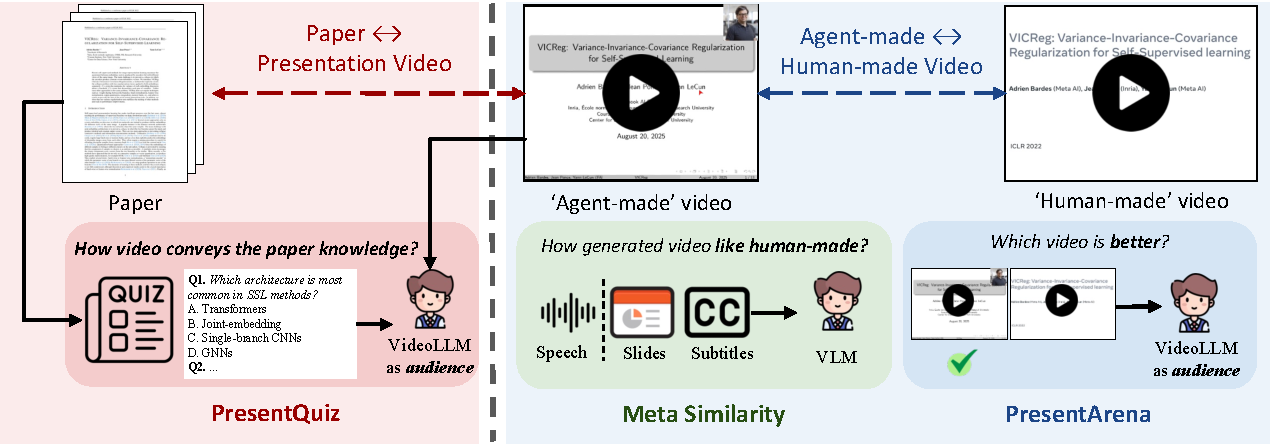
\includegraphics[width=1\linewidth]{figure/eval.pdf}
    \caption{\textbf{Overview of evaluation metrics.} We propose three metrics that systematically evaluate academic presentation video generation from the perspective of the relationship between the generated video and \textbf{(i)} the original paper and \textbf{(ii)} the human-made video.}
    \label{fig:eval}
    \vspace{-0.2\baselineskip}
\end{figure}
% \kevin{Furthermore, to ablate XXX, we devise a X (talking head), Y (cursor), Z (slide) to study gain by individual component, in appendix. Notably, we also include the human studies}
% the information coverage rate of the generated presentation video in respect to the original presentation video length.
% \noindent\textbf{Test-of-Memory.} \textit{-- How video influence its academic impact?} Inspired by live conference settings, this metric tests whether viewers can recall a work and formulate an appropriate question after watching the presentation, thereby assessing memorability and academic impact. For each method, we randomly sample four generated presentation videos and extract a ten-second clip from each. For every clip, we draw one question from \textit{PresentQuiz} associated with the corresponding paper. We then prompt a VideoLLM to watch the four clips. Next, we querry the model with an author portrait randomly sampled from the same set and ask it to select the question that best matches that author’s work. Overall accuracy is reported as the metric, with higher values indicating stronger memorability and question-elicitation ability.

% to systematically xxx, we devise the following metrics:
% (i) (Human-like) Similarity: how human-like with ground-truth video, how model prediction, but not a prefect; video, slides+subtitle, speech
% (ii) PresentArena: which one is better 
% (iii) PresentQuiz: Motivated by the purpose of presentation, a good presentation should XXX, thus we design a 
% (iv) Present-IP: identifier, academic IP

% [add figure--iii/iv]
